\documentclass[10pt]{article}
\usepackage[utf8]{inputenc}
\usepackage[a4paper]{geometry}

\usepackage{pdfpages}
\usepackage[colorlinks=true, urlcolor=cyan]{hyperref}

\usepackage{listings}
\usepackage{xcolor}

\definecolor{mygreen}{rgb}{0,0.6,0}
\definecolor{mygray}{rgb}{0.5,0.5,0.5}
\definecolor{mymauve}{rgb}{0.58,0,0.82}

\lstset{ %
  language=C++,								  % the language of the code
  backgroundcolor=\color{black!5}, % set backgroundcolor,   % choose the background color; you must add \usepackage{color} or \usepackage{xcolor}
  basicstyle=\footnotesize,        % the size of the fonts that are used for the code
  breakatwhitespace=false,         % sets if automatic breaks should only happen at whitespace
  breaklines=true,                 % sets automatic line breaking
  captionpos=b,                    % sets the caption-position to bottom
  commentstyle=\color{mygreen},    % comment style
  deletekeywords={...},            % if you want to delete keywords from the given language
  escapeinside={\%*}{*)},          % if you want to add LaTeX within your code
  extendedchars=true,              % lets you use non-ASCII characters; for 8-bits encodings only, does not work with UTF-8
  frame=single,	                   % adds a frame around the code
  keepspaces=true,                 % keeps spaces in text, useful for keeping indentation of code (possibly needs columns=flexible)
  keywordstyle=\color{blue},       % keyword style
  otherkeywords={*,...},           % if you want to add more keywords to the set  
  numbers=left,                    % where to put the line-numbers; possible values are (none, left, right)
  numbersep=7pt,                   % how far the line-numbers are from the code
  numberstyle=\tiny\color{mygray}, % the style that is used for the line-numbers
  stepnumber=1,                    % the step between two line-numbers. If it's 1, each line will be numbered
  rulecolor=\color{black},         % if not set, the frame-color may be changed on line-breaks within not-black text (e.g. comments (green here))
  showspaces=false,                % show spaces everywhere adding particular underscores; it overrides 'showstringspaces'
  showstringspaces=false,          % underline spaces within strings only
  showtabs=false,                  % show tabs within strings adding particular underscores
  stringstyle=\color{mymauve},     % string literal style
  tabsize=4,	                   % sets default tabsize to 4 spaces
  title=\lstname                   % show the filename of files included with \lstinputlisting; also try caption instead of title
}

\lstdefinestyle{customc}{
  belowcaptionskip=1\baselineskip,
  breaklines=true,
  frame=L,
  xleftmargin=\parindent,
  language=C++,
  showstringspaces=false,
  basicstyle=\footnotesize\ttfamily,
  keywordstyle=\bfseries\color{green!40!black},
  commentstyle=\itshape\color{purple!40!black},
  identifierstyle=\color{blue},
  stringstyle=\color{orange},
}

\lstset{escapechar=@,style=customc}

\title{2015-2016 ACM-ICPC Nordic Collegiate Programming Contest (NCPC 2015)} % // is line break
\author{Chun-Hung Tseng}
\date{\today}

% Use this tag to surround the entire document, a must
\begin{document} 

\begin{titlepage}
\maketitle
\end{titlepage}

%By default, the paragraphs are indented by 1.5 times the point size of the current font. Also, there is no extra blank space inserted between the paragraphs. In the sections below is described how to change that.

%A
\includepdf[pages={3,4}]{problem_statement.pdf}

\section*{Problem A}

This is a very interesting problem, which I got 12 WA during virtual participation on Codeforces. Draw the diagram out for the ths problem, you will realise that this is a problem about tree diameter and radius pretty quickly. \\

You are given some forests to start with, and you have to add one edge for each tree in the forest to connect all of them together eventually, such that the forest will become a tree, where the furthest two leaves are of the shortest distance.\\ 

Finding the diameter and radii is the part that got me 12 WA, because I didn't implement it the right way for the first 10+ attempts. Here is a great article on \href{http://codeforces.com/blog/entry/17974}{Codeforces} that have great explanations on this. \\

Let's denote $D$ for the largest diameter of all trees in the forest, $A$ for the largest radius, $B$ for the second-largest radius(if exists), and $C$ for the third-largest radius of all trees(if exists). The answer will be $max(D, A+B+1, B+C+2)$. Because the furthest two leaves are of the closest distance wiil be determined by the longest "chains" in the trees after connecting all of them together, and we can see if we connect all trees on to the center of the longest diameter, we can minimize the distance of the furthest leaves\\

\lstinputlisting[language=c++]{A/main.cpp}

\newpage

%C
\includepdf[pages={7}]{problem_statement.pdf}

\section*{Problem C}

\lstinputlisting[language=c++]{C/main.cpp}

\newpage

%D
\includepdf[pages={9}]{problem_statement.pdf}

\section*{Problem D}

\lstinputlisting[language=c++]{D/main.cpp}

\newpage

%E
\includepdf[pages={11}]{problem_statement.pdf}

\section*{Problem E}

\lstinputlisting[language=c++]{E/main.cpp}

\newpage

%G
\includepdf[pages={15,16}]{problem_statement.pdf}

\section*{Problem G}

\lstinputlisting[language=c++]{G/main.cpp}

\newpage

\end{document}
